%
% Based on the culmus-test, culmus-ex and hebhello examples from
% culmus-latex-0.7-r1 from
% http://sourceforge.net/projects/ivritex/files/culmus-latex/
%
\documentclass[12pt]{article}
\usepackage[utf8x]{inputenc}
\usepackage[hebrew,english]{babel}
\usepackage{culmus}
\usepackage[yyyymmdd]{datetime}
\usepackage{amsmath,amssymb,amsthm}
\usepackage{graphicx}
\usepackage{textcomp}
%general:
%Box and color definitions:
%--------------------------
\newenvironment{ColorBoxedminipage}
{\begin{minipage}} {\end{minipage}}
%{\begin{Sbox}\begin{minipage}}
%{\end{minipage}\end{Sbox}\fcolorbox{Blue}{White}{\TheSbox}}

%General definitions:
%-------------------
\newcommand{\etal}{{\em {et al.}}}
\newcommand{\B}[1]{\mathbf{#1}}
\newcommand{\df}{\triangleq}
\newcommand{\norm}[1]{\left\Vert#1\right\Vert}
\newcommand{\abs}[1]{\left\vert#1\right\vert}
\newcommand{\RE}{\operatorname{Re}}
\newcommand{\IM}{\operatorname{Im}}
\newcommand{\sgma}[3]{\sum\limits_{{#1}={#2}}^{#3}}
\newcommand{\Brace}[1]{\left\{{#1}\right\}} %Braces
\newcommand{\Brack}[1]{\left({#1}\right)} %Brackets
\newcommand{\sBrack}[1]{\left[{#1}\right]} %square Brackets

%\newcommand{\ip}[2]{{\langle{#1},{#2}\rangle}} %inner-product
\newcommand{\ipLW}[3]{{\langle{#1},{#2}\rangle}_{{#3}}} %weighted inner-product

\newcommand{\Tr}[1]{Tr\Brack{#1}}
\newcommand{\Mtr}[2] %short notation for 2x1 Matrix.
{\begin{bmatrix}
  #1 \\
  #2
\end{bmatrix}}
\newcommand{\cMtr}[2] %short notation for 2x1 Matrix with curves.
{\left(
\begin{array}{c}
    {#1} \\
    {#2} \\
\end{array}
\right)}
\newcommand{\Mtrs}[2] %short notation for 2x1 Matrix star (adjoint)
{\begin{bmatrix}
  #1 &
  #2
\end{bmatrix}}
\newcommand{\Mtrt}[3] %short notation for 3x1 Matrix.
{\begin{bmatrix}
  #1 \\
  #2 \\
  #3
\end{bmatrix}}

\newcommand{\Cases}[4]{
\left\{
\begin{tabular}{lcl}
    $#1$ & $=$ & $#2$\\
    $#3$     & $=$ & $#4$
\end{tabular}
\right. }

\newcommand{\und}{\underline} %How lazy can I get?
\newcommand{\ovr}{\overline}
\newcommand{\conj}[1]{{#1}^\ast} %Conjugation


\newcommand{\er}[1]{{(\ref{#1})}} %equation reference

\newtheorem{Lemma}{Lemma}{}
\newtheorem{Prop}{Proposition}{}
\newtheorem{theorem}{Theorem}{}


\newenvironment{alg}[5]
{
\begin{figure}[htbp]
\begin{center}
\fbox{
  \begin{ColorBoxedminipage}{13cm}
%    \leftline{\color{Black}\bf {#1}}
    {#4}
   \end{ColorBoxedminipage}
   }
\end{center}
  \bcaptionff{#1}{#2}{}{#3}
  \label{#5}
\end{figure}
}{}

%Just body, caption and label.
\newenvironment{algo}[3]
{
\begin{figure}[htbp]
\begin{center}
\fbox{
  \begin{ColorBoxedminipage}{7.5cm}
%    \leftline{\color{Black}\bf {#1}}
    {#1}
   \end{ColorBoxedminipage}
   }
\end{center}
  \caption{#2}
  \label{#3}
\end{figure}
}{}

\newenvironment{BOX}[1]
{
\begin{center}
\fbox{
  \begin{ColorBoxedminipage}{16cm}
%    \leftline{\color{Black}\bf {#1}}
    {#1}
   \end{ColorBoxedminipage}
   }
\end{center}
}{}

\newcommand\vecnot[1]{\boldsymbol{#1}}
\newcommand\optvecnot[1]{\vecnot{#1}_{opt}}

\usepackage{amsmath}
\DeclareMathOperator*{\argmax}{arg\,max}
\DeclareMathOperator*{\argmin}{arg\,min}

%Configuration-------------------------------------------------------------
\setlength{\parskip}{0.2cm}
\setlength{\parindent}{0cm}
\addto{\captionshebrew}{
    \renewcommand{\refname}{Bibliography}
    \renewcommand{\contentsname}{Table of Contents}
}
\newcommand{\printdate}[3]{{%
\day=#1\relax\month=#2\relax\year=#3\relax\today}}

\title{
\begin{otherlanguage}{hebrew}
עיצוב אלומה מרחבי מבוסס משוב לעיבוד אותות אקוסטיים
\end{otherlanguage}
\\
Feedback Based Spatial Beamforming With Applications to Acoustic Signal Processing
}
\author{
Yehezkel Karo Itay\\[1cm]{Supervisor: Prof. Cohen Israel}\\{external supervisor: Dr. Dvorkind Tsvi}
}
\title{Feedback Based Spatial Beam-forming with Applications to Acoustic Signal Processing}
\begin{document}
\maketitle
\section*{Introduction}
Uniform linear array (ULA) processing in the spatial domain is similar to time domain finite-impulse-response (FIR) filtering (e.g. \cite{van1988beamforming}).
The similarity arises because temporal FIR's input is composed of equally time-spaced samples and the ULA's input is obtained from equally spatially-spaced samples of the impinging wavefront.
Both temporal FIR and ULA filtering assign weights to each sample in order to achieve a desired temporal/spatial response.
From time domain filter design theory, it is well known that infinite impulse response (IIR) filters attain certain advantages over FIR filtering.
A natural question to consider is ``what is the array structure in spatial domain which is analogous to IIR filtering in the time domain?''.
The motivation for finding an IIR equivalent in the spatial domain is obvious:
\begin{itemize}
\item
{
Increased degrees of freedom over conventional array processing to control the array response.
}
\item
{
Substantially lower number of taps (smaller number of array elements and reduced array aperture) is required for obtaining a desired response in comparison to an FIR based design. This, naturally, results in cost-efficient array.
}
\end{itemize}
In his PhD thesis \cite{wen2013array}, Wen presented the same question. In his work two approaches were suggested for achieving ``spatial-IIR'' filtering.
First was to use shifted-sub-arrays, in order to approximate the auto-regressive part of the filter.
In practice, this approximation is equivalent to a truncated response of the IIR filter thus obtaining only an FIR implementation.
The second approach in \cite{wen2013array}, was to estimate the DOA of the impinging signal and approximate the auto-regressive part of the filter by temporal processing.
The latter approach is speculated to be very sensitive to DOA estimation errors; and it is not clear how one may extend this approach to multiple speakers scenario.
Additional works \cite{Madanayake2008ABeamformer,Madanayake2009SystolicWDFs,Madanayake2008AFilters,Bruton2003Three-dimensionalBanks,Ward1986ABeamforming,Joshi2012SynthesisApplications} consider a different approach of 2-D spatio-temporal filtering. In particular, the wavefront is viewed as a two dimensional signal, and the processing is done by performing IIR filtering in the time domain, but only FIR filtering (using a finite number of sensors) is performed in the spatial domain.
As can be seen in \cite{Bruton2003Three-dimensionalBanks}, the obtained 2-D filter is not ideal, causing imperfections in the overall spatial response.
\\
In this work we propose spatial-IIR filtering. As time-domain filter design relies on feeding back the filter's input with a combination of its taps, our approach relies on spatial feedback of received array signals back to the transmitter.
In the context of acoustic signal processing, a cooperative speaker will hold an electronic or acoustic transponder. 
Thus, the received signals at a microphone array will consist of the direct speech signal of the speaker, and a feedback signal which was recorded by the array at a previous time epoch (see Fig. \ref{fig:SignalModel}). 
Naturally, this suggested approach requires a cooperative speaker/source but, as will be explained, spatial-only-IIR filtering will be achieved by this scheme.
Comparing to \cite{wen2013array}, our method solves the main issues of both suggested approaches, achieving spatial IIR processing of multiple speaker scenarios.
\begin{figure}[!ht]
\begin{center}
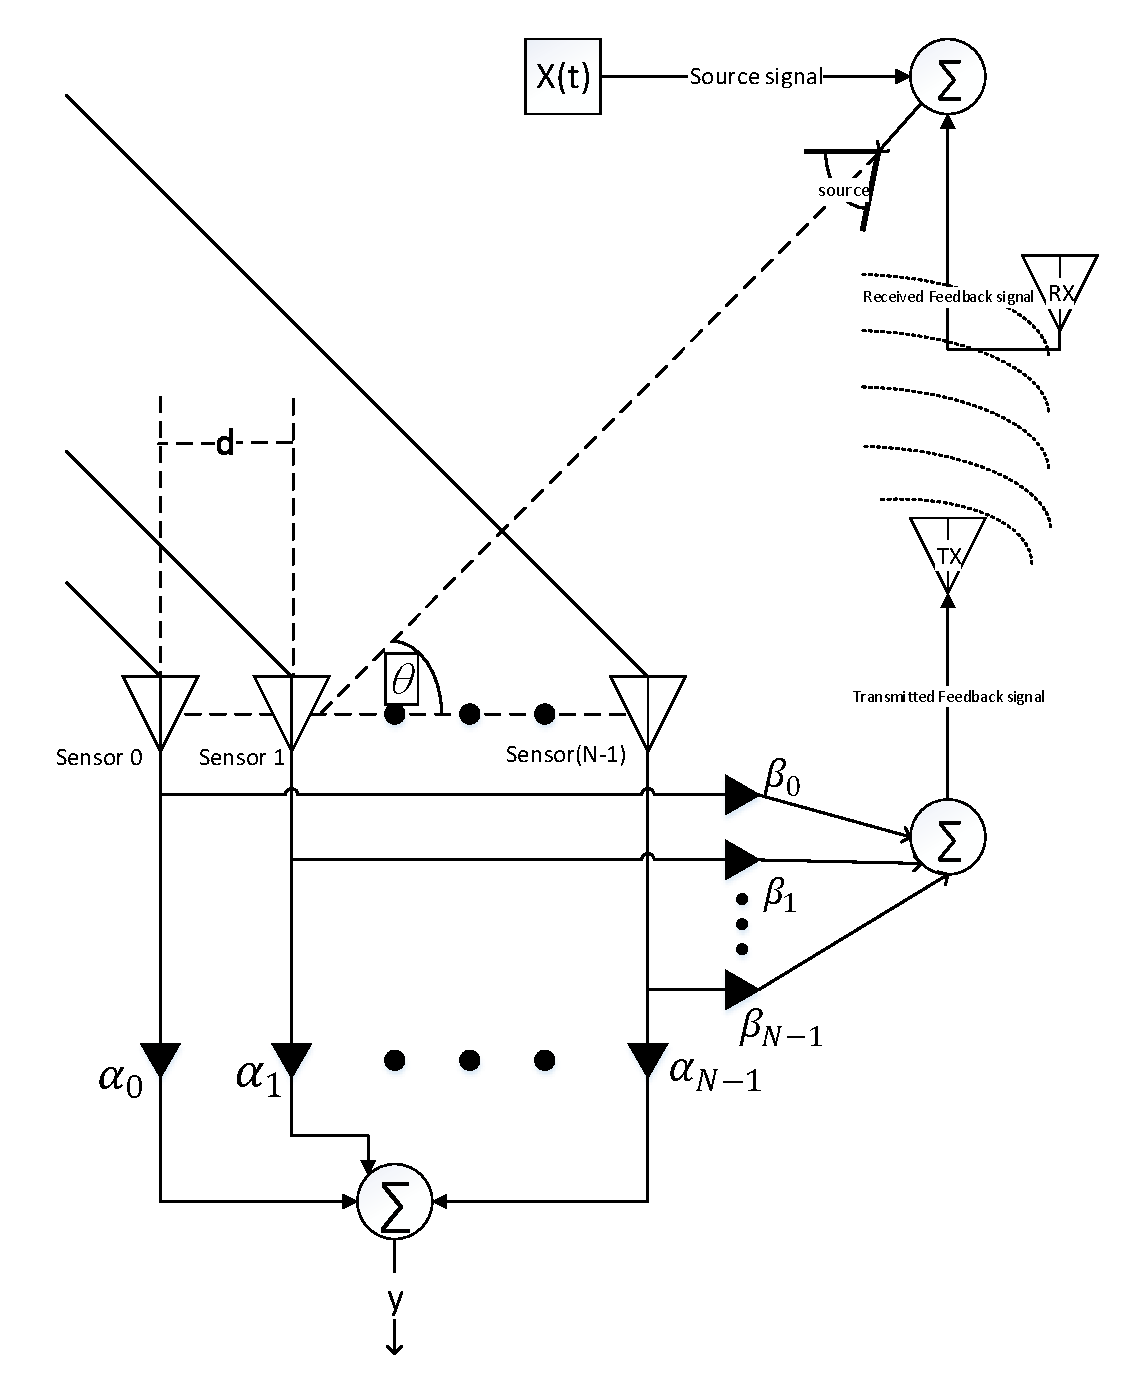
\includegraphics[width=0.5\textwidth]{./Media/SpatialIIR-diagram/SpatialIIR_VER4.pdf}
\caption
{
Proposed system: A far field source is received by an array. 
The received signal is also retransmitted back to the source. 
The latter has a transponder which feeds the signal back to the array.
}
\label{fig:SignalModel}
\end{center}
\end{figure}
It can be shown that with this approach one gets the transfer function of the overall system
$$
\ensuremath{
y_{\theta}^{\mathcal{F}}(\omega) 
=
\frac
{
\vecnot{\alpha}^{T}
\vecnot{d}_{\theta}
exp\left(-j\tau\right)
}
{
1
-
\vecnot{\beta}^{T}\vecnot{d}_{\theta}
exp\left(-j\tau\right)
}
x^{\mathcal{F}}(\omega)
}
$$
where $ x $ is the source signal, $ y $ is the beam-former output, $ \theta $ is the direction-of-arrival (DOA) angle of the received signal, $ \vecnot{\alpha},\vecnot{\beta} $ are user-controlled coefficient vectors, $\vecnot{d}_{\theta}$ is the steering vector, $ \tau_{pd}$ and $ \tau_{tx} $ are the propagation delay from the source to the reference sensor and the feedback transmission delay respectively.
$^{T}$ stands for the transpose operator and the super-script $ ^{\mathcal{F}} $ represents the Fourier transform. 
The existence of a $ \theta $ dependent denominator in the transfer function proves IIR filtering is achieved for cooperative speakers.
\section*{Research goals}
In this work we will investigate and develop methods of choosing the coefficients $ \vecnot{\alpha} $ and $ \vecnot{\beta} $ when a desired beam-pattern, $ H_{d}(\theta)$, is to be approximated. We will examine the outcome of partial knowledge of the propagation delays $\tau_{pd},\tau_{tx}$ and their influence on the stability of the filter. Another possible direction of research is to consider a more realistic reverberant channels which are common in acoustical environments, rather than the simple one-tap channel presented here. Simulations of dynamic spatial filtering of multi-speakers will be presented and compared to other conventional methods such as the classical delay and sum beam-former. Finally, we intend to implement the above suggested system.
\small
{
\bibliographystyle{unsrt}
\bibliography{./Modules/Mendeley,./Modules/LocalBib}
}
\end{document}